\chapter{Ergebnisse}

In den folgenden Abschnitten werden die Ergebnisse dieser Arbeit vorgestellt.
Die in Kapitel \ref{ch:festkoerpermodelle} vorgestellten Festkörper-Modelle werden für mikroskopische, zweidimensionale, kubische Festkörpersysteme aus vier Gitterplätzen untersucht.
Vielteilchenzustände werden in erster und Operatoren in zweiter Quantisierung dargestellt.
Numerische Diagonalisierungen von Matrizen werden mit der Funktion //eig von octave// durchgeführt.

\section{Untersuchung eines Festkörpersystems im Tight-Binding-Modell}
\label{sec:untersuchungtb}

Dieser Abschnitt beschäftigt sich mit der Dynamik eines Festkörpersystems, bestehend aus vier Niveaus, die jeweils einen Gitterplatz repräsentieren, und einem bzw. zwei Elektronen (im Folgenden abgekürzt mit 4N1E bzw. 4N2E),
im Tight-Binding-Modell analysiert. Das 4N1E-System wird ist in Abbildung \ref{fig:vierniveausystem} mit beispielhafter Besetzung skizziert.

\begin{figure}
  \centering
  \includegraphics[height = 4cm]{Graphiken/vier_niveau_system.pdf}
  \caption{Skizze des 4N1E-Systems mit beispielhafter Besetzung $\ket{3}$. Die waagerechten Striche stellen die Niveaus dar, die eingekreisten Zahlen die Nummer des Gitterplatzes, der rot gefärbte Kreis das Elektron
  und die Pfeile die möglichen Sprünge des Elektrons aus der dargestellten Besetzung in Abhängigkeit von $J$.}
  \label{fig:vierniveausystem}
\end{figure}

Das eine Elektron kann abhängig von der Wechselwirkungs-Konstante $J$ waagerecht oder senkrecht zwischen den Gitterplätzen springen.
Der Hilbertraum des 4N1E-Systems setzt sich aus vier Basis-Zuständen, bei denen sich das Elektron jeweils auf einem der vier Gitterplätze befindet, zusammen und ist daher vierdimensional.
Um die Dynamik zu analysieren werden zuerst die Basis-Zustände aufgestellt, daraus die vierdimensionale Hamilton-Matrix bestimmt und mit Hilfe dieser die Schrödingergleichung \ref{eqn:schroedingergleichung} gelöst.

Die Basis-Zustände werden in der Konvention
\begin{align}
  \ket{i} = \ket{f_i(x)}
  \label{eqn:4N1Ezustandsvorschrift}
\end{align}
dargestellt. Dabei gibt die Funktion $f_i(x)$ die Nummer des Gitterplatzes an, auf dem sich das Elektron $x$ befindet.
Der Hamiltonian des Systems ist in Gleichung \eqref{eqn:hamiltontb} in zweiter Quantisierung angegeben, wobei periodische Randbedingungen in der Summe impliziert werden.
In Tabelle \ref{tab:4N1Ehamiltonmatrix} ist die Matrixdarstellung des Hamilton-Operators, die sich aus Gleichung \eqref{eqn:matrixelemente} ergibt, zu sehen.
Mit dieser Darstellung wird die Schrödingergleichung \eqref{eqn:schroedingergleichung}, die durch den Hamilton-Operator $H$ festgelegt ist, aufgestellt.
Da dieser zeitunabhängig ist, ergibt sich die stationäre Schrödingergleichung \eqref{eqn:statschroedinger}, welche durch Diagonalisieren des Hamilton-Operators $H$ mit analytisch gelöst wird.
Die berechneten Energie-Eigenwerte $E_k/J$ und die Koeffizienten $\alpha_{i,k}$ der generierten Eigenzustände $\Psi_k$ sind in Tabelle \ref{tab:4N1Eeig} aufgelistet.
Die Eigenzustände ergeben sich aus der Linearkombination
\begin{align}
  \Psi_k = \sum_i \alpha_{i,k} \ket{i}.
  \label{eqn:linkomb}
\end{align}
Da das Betragsquadrat des Koeffizienten $\alpha_{i,k}$ der Besetzungswahrscheinlichkeit $P_i \in [0,1]$ für den i-ten Basis-Zustand des Systems im Eigenzustand $Psi_k$ entspricht,
ist an die Linearkombination \eqref{eqn:linkomb} die Normierungsbedingung
\begin{align}
  \sum_i \lvert \alpha_{i,k} \rvert^2 = 1.
  \label{eqn:tbnb}
\end{align}
geknüpft.

\begin{table}[h]
  \centering
  \caption{Analytisch berechnete Eigenwerte $E_k/J$ und zugehörige Koeffizienten $\alpha_{i,k}/0.5$ der Eigenzustände $\Psi_k$ des 4N1E-Systems.}
  \begin{tabular}{S[table-format=1.0] S[table-format=2.0] S[table-format=1.0] S[table-format=1.0] S[table-format=1.0] S[table-format=2.0]}
    \toprule
    {$k$} & {$E_k/J$} & {$\alpha_{1,k}/0.5$} & {$\alpha_{2,k}/0.5$} & {$\alpha_{3,k}/0.5$} & {$\alpha_{4,k}/0.5$}\\
    \midrule
    0 & -2 & 1          & 1          & 1                  & 1                  \\
    1 & 0  & $\sqrt{2}$ & 0          & \text{$-\sqrt{2}$} & 0                  \\
    2 & 0  & 0          & $\sqrt{2}$ & 0                  & \text{$-\sqrt{2}$} \\
    3 & 2  & 1          & -1         & 1                  & -1                 \\
    \bottomrule
  \end{tabular}
  \label{tab:4N1Eeig}
\end{table}

%Die einzige Quantenzahl, in denen sich die Basis-Zustände des 4N1E-Systems unterscheiden, ist die Nummer $i$ des Gitterplatzes, an welchem das Elektron positioniert ist.
%Da alle Gitterplätze jeweils zwei direkte Nachbarn besitzen, die sich bis auf die Nummer $i$ nicht unterscheiden,
%ist die Besetzungswahrscheinlichkeit des Elektrons in den Eigenzuständen, die sich aus nicht-entarteten Eigen-Energien ergeben, gleichmäßig auf alle vier Basis-Zustände bzw. Niveaus aufgeteilt.
%Aus der Normierungsbedingung \eqref{eqn:tnbn} folgt daher für diese Eigenzustände des Systems
%\begin{align}
%  P_{i,k} = \lvert \alpha_{i,k} \rvert^2 = 0.25.
%  \label{eqn:BesetzungRot}
%\end{align}
%Das ist für die berechneten Eigenzustände $v_0$ und $v_3$ der Fall. Für die Eigenzustände zu entarteten Energie-Eigenwerten, hier $v_1$ und $v_2$ zur Energie $E_1 = E_2 = 0$, können mehrere verschiedene
%Basen gewählt werden, sodass Gleichung \eqref{eqn:BesetzungRot} nicht zwangsläufig gilt. Der physikalische Grund dafür ist, dass das Elektron bei hinreichender Energie einen Zustand,
%der sich aus einer Linearkombination der beiden Eigenzustände $v_1$ und $v_2$ ergibt, besetzt.

Um den Einfluss einer Elektron-Elektron-Wechselwirkung im Vierniveau-System zu untersuchen, wird ein weiteres Elektron ergänzt.
In dem 4N2E-System sind die waagerechten oder senkrechten Sprünge der Elektronen zwichen den Gitterplätzen nicht mehr beliebig möglich,
falls die beiden Elektronen auf benachbarten Gitterplätzen sitzen, da die Doppelbesetzung eines Niveaus durch das Pauliprinzip verhindert wird.
Für das 4N2E-System ergeben sich insgesamt
\begin{align}
  \binom{d_{\text{1e}}}{N_e} = \binom42 = 6 (footnote)
\end{align}
verschiedene Zustände, wobei $d_\text{1e}$ die Hilbertraum-Dimension des 4N1E-System und $N_e$ die Anzahl an Elektronen ist.
Die Eigenenergien setzen sich jeweils additiv aus zwei wegen des Pauliprinzips unterschiedlichen Eigenenergien des 4N1E-Systems, siehe Tabelle \ref{tab:tbeigene1}, zusammen.
In Tabelle \ref{tab:4N2Eeigenwerte} sind die addierten Eigenenergien für das 4N2E-System aufgelistet.
Aus der zweifachen Entartung der Energie $E = 0$ im 4N1E-System folgt unter anderem die Entartung des Grundzustands im 4N2E-System.

\begin{table}[h]
  \centering
  \caption{Additiv aus den Eigenenergien des 4N1E-Systems in Tabelle \ref{tab:4N1Eeig} berechnete Eigenenergien des 4N2E-Systems in Einheiten von $J$.}
  \begin{tabular}{S[table-format=2.0] S[table-format=2.0] S[table-format=1.0] S[table-format=1.0] S[table-format=1.0] S[table-format=1.0]}
    \toprule
    {$E_0/J$} & {$E_1/J$} & {$E_2/J$} & {$E_3/J$} & {$E_4/J$} & {$E_5/J$}\\
    \midrule
    -2 & -2 & 0 & 0 & 2 & 2 \\
    \bottomrule
  \end{tabular}
  \label{tab:4N2Eeigenwerte}
\end{table}

\section{Untersuchung eines halbgefüllten Festkörpersystems im Hubbard-Modell}
\label{sec:untersuchunghubb}

In diesem Abschnitt wird die Dynamik eines Festkörpersystems, bestehend aus vier Gitterplätzen und acht Niveaus, im Hubbard-Modell untersucht.
Jeder Gitterplatz besitzt zwei Niveaus, die sich jeweils in der Spinmagnetquantenzahl $\sigma$ unterscheiden.
Auf jeweils vier Niveaus mit äquvalenter Spinausrichtung sind zwei Elektronen verteilt, sodass das System (im Folgenden mit 8N4E abgekürzt) insgesamt halbgefüllt ist.
In Abbildung \ref{fig:hubbsystem} ist eine Skizze des Systems mit beispielhafter Elektronenbesetzung abgebildet.

\begin{figure}
  \centering
  \includegraphics[height = 7cm]{Graphiken/hubb_system.pdf}
  \caption{Skizze des 8N4N-Systems mit beispielhafter Besetzung $\ket{1,4;2,4}$. Die blau gestrichelten Kreise umfassen jeweils einen Gitterplatz mit zwei Niveaus.
  Der jeweils näher am Zentrum des Systems eingezeichnete waagerechte Strich stellt das Spin-Down- und der jeweils außen eingezeichnete waagerechte Strich das Spin-Up-Niveau des jeweiligen Gitterplatzes dar. Die roten Pfeile beschreiben die Elektronen mit ihrer Spinausrichtung.
  Doppeltbesetzte Gitterplätze beinhalten das Potential $U$ und die eingezeichneten Elektronen können jeweils abhängig von $U$ und $J$ in Pfeilrichtung springen.}
  \label{fig:hubbsystem}
\end{figure}

Die Elektronen können unter Beachtung des Pauliprinzips waagerecht oder senkrecht zwischen den Gitterplätzen auf dem jeweiligen Spin-Niveau springen.
Das 8N1E-System besteht effektiv aus zwei gekoppelten 4N2E-Systemen mit unterschiedlicher Spinausrichtung und
beinhaltet daher $6 \cdot 6=36$ Basis-Zustände bzw. umfasst einen 36D-Hilbertraum.
Mit Hilfe der Kurzschreibweise der Vielteilchenzustände \eqref{eqn:vtdarstellung1quantkurz} werden die Basis-Zustände des Systems in erster Quantisierung in dem Schema
\begin{align}
  \ket{i} = \ket{f_i(\uparrow_1),f_i(\uparrow_2); f_i(\downarrow_1),f_i(\downarrow_2)}
  \label{eqn:hubbzustandsvorschrift}
\end{align}
dargestellt. Dabei ist $f_i(x_\alpha)$ eine Funktion, welche den Ort des Elektrons $x_\alpha$ im i-ten Basis-Zustand des Systems angibt.
In der Bezeichnung des Elektrons $x_\alpha$ stellt $x$ die Spinausrichtung und der Index $\alpha$ die Nummer des Elektrons dar, wobei die Elektronen eines Spinniveaus gegen den Uhrzeigersinn und beginnend beim Gitterplatz $1$ durchnummeriert werden.
Diese Konvention führt automatisch dazu, dass der zweite Eintrag einer Spinausrichtung in der Darstellung der Zustände \eqref{eqn:tbzustandsvorschrift} größer als der erste ist.
Die Darstellungen der $36$ Zustände aus Gleichung \eqref{eqn:hubbzustandsvorschrift} sind im Anhang in Tabelle \ref{tab:hubbzustandsvorschrift} aufgelistet.
Der Hamiltonoperator des 8N4E-Systems ist in Gleichung \eqref{eqn:hamiltonhubb} angegeben, wobei erneut periodische Randbedingungen in der Summe impliziert werden.
Um die Schrödingergleichung für das System zu lösen, wird analog zur Lösung der Schrödingergleichung des 4N1E-Systems in Abschnitt \ref{sec:untersuchungtb} vorgegangen.
Die $36 \times 36$ -Matrix des Hamilton-Operators ist in Tabelle \ref{tab:hubbhammatrix} abgebildet.
Der Vorfaktor $J$ des Tight-Binding-Terms \eqref{eqn:hubbsys} bestimmt die Nichtdiagonalelemente und der
Vorfaktor $U$ des Elektronen-Potentialterms die Diagonalelemente der Hamilton-Matrix.
Die vier niedrigsten Eigenwerte in Einheiten von $J$ sind im Anhang in Tabelle \ref{tab:eigenwerte} für diverse $U/J$ aufsteigend aufgelistet und in Abbildung \ref{fig:eplot} gegen $U/J$ graphisch aufgetragen.

\begin{figure}
  \centering
  \includegraphics{build/Hubb_eplot.pdf}
  \caption{plot.}
  \label{fig:eplot}
\end{figure}

Im Grenzfall $U/J = 0$ wechselwirken die Spin-Up-Elektronen nicht mit den Spin-Down-Elektronen, sodass sich die 36 Eigenenergien des 8N4E-Systems additiv aus den
Eigenenergien des 4N2E-Systems zusammensetzen. Der systematische Unterschied zur Addition der Eigenenergien in Kapitel \ref{sec:untersuchungtb} ist, dass hier alle
Eigenenergien miteinander kombiniert werden können. Das ist darin begründet, dass sich die Elektronen der 4N2E-Systeme um eine zusätzliche Quantenzahl,
die Spinausrichtung $\sigma$, unterscheiden und somit keine Pauliabstoßung zwischen den gekoppelten 4N2E-Systemen existiert.
Aus den Kombinationen der zweifach entarteten Grundzustandsenergie des 4N2E-Systems aus Tabelle \ref{tab:4N2Eeigenwerte} ergibts sich die vierfach entartete Grundzustandsenergie des Gesamtsystems $E/J = -4$ für $U/J = 0$.
Dies ist auch in Abbildung \ref{fig:eplot} erkennbar, die Kurven der vier niedrigsten Eigenenergien schneiden die Abzisse bei $E/J = -4$.
Der Verlauf der Eigenenergie $E_3$ besitzt einen Knick, der durch den Differenzenquotienten zweiter Ordnung an der Stelle $U/J = 2.44949$ lokalisiert wird.
Die Ursache für diesen Knick wird in Kapitel \ref{sec:spin} erklärt.

\section{Vergleich des oberen Potential-Grenzfalls im halbgefüllten Hubbard-Modell mit dem Heisenberg-Austausch-Modell}

In diesem Kapitel wird der Potential-Grenzfall $U\to\infty$ für das 8N4E-System im Hubbard-Modell analysiert. Dafür wird die Grundzustandsenergie des Systems im Hubbardmodell für steigendes $U$ untersucht und mit der Grundzustandsenergie des Systems im Heisenberg-Austausch-Modell
verglichen, da für $U\to\infty$ ein Übergang vom halbgefüllten Hubbard-Modell in das Heisenberg-Austausch-Modell erwartet wird.

Die Grundzustandsenergie des Heisenberg-Austausch-Modells in Einheiten von $J$
\begin{align}
  \frac{E_\text{0,spin}}{J} = - \eta \frac{t}{J} = - \eta \frac{4J}{U}
  \label{eqn:e0spin}
\end{align}
folgt aus der Relation \eqref{eqn:spint}. Dabei ist $\eta$ eine Konstante, die im Heisenberg-Austausch-Modell und gegebenenfalls auch im Hubbard-Modell bestimmt werden kann.
Die Erwartung ist, dass die Grundzustandsenergie des Hubbard-Modells im Grenzfall $U \to \infty$ in den Wert \eqref{eqn:e0spin} übergeht,
\begin{align}
  \lim\limits_{U \to \infty} E_\text{0,hubb} = E_\text{0,spin}.
\end{align}
Daraus resultiert eine Geradengleichung für den natürlichen Logarithmus der Grundzustandsenergie in Abhängigkeit vom natürlichen Logarithmus des Potentials,
\begin{align}
  \ln{\frac{E_\text{0,hubb}}{J}} = -\ln{\frac{U}{J}} + \ln{4 \eta'}.
  \label{eqn:loge0hubb}
\end{align}
Um diese zu überprüfen, sind in Abbildung \ref{fig:loglog} die numerisch berechneten Grundzustandsenergien $E_\text{0,hubb}/J$ in einem Log-Log-Plot gegen das Potential $U/J$ aufgetragen.

\begin{figure}
  \centering
  \includegraphics{build/Hubb_Grenz_Plot.pdf}
  \caption{plot.}
  \label{fig:loglog}
\end{figure}

Der Verlauf von $\ln{E_\text{0,hubb}/J}$ ist für $U \to 0$ gekrümmt und geht für steigendes $U$ in eine Gerade über, wie erwartet.
Der natürliche Logarithmus der Grundzustandsenergie wird für große $U$, hier insgesamt 10001 Potentialwerte in dem Abstand $\Delta U/J = 1$ von $U/J = \num{40000}$ bis $U/J = \num{50000}$,
linear approximiert. Die Approximationsgerade ist ebenfalls in Abbildung \ref{fig:loglog} zu sehen. Zur Geradengleichung
\begin{align}
  \ln{\frac{E_\text{0,hubb}}{J}} = m \ln{\frac{U}{J}} + n
  \label{eqn:loge0hubbgerade}
\end{align}
werden die Regressionsparameter
\begin{align}
  m & = -1 + \num{3.4(8)e-08}  & n & = 2.484906
  \label{eqn:regressionsparameter}
\end{align}
berechnet. Die relative Abweichung der Steigungen beim Koeffizientenvergleich von Gleichung \eqref{eqn:loge0hubb} mit \eqref{eqn:loge0hubbgerade} ist mit
\begin{align}
  \Delta m_\text{rel} = 1- \frac{m}{-1} = \SI{3.4(8)e-06}{\percent}
\end{align}
meines Erachtens nach gering. Die Proportionalität $E \propto U^{-1}$ für $U \to \infty$ ist daher bestätigt.
Der Fehler des Abzissenabschnittes $n$ in \eqref{eqn:regressionsparameter}, der in der Regression berechnet wird, liegt in der Größenordnung $10^{-8}$ und wird daher vernachlässigt.
Aus dem Koeffizientenvergleich von Gleichung \eqref{eqn:loge0hubb} mit \eqref{eqn:loge0hubbgerade} folgt der Wert der Konstante
\begin{align}
  \eta' = 2.999998
  \label{eqn:eta1}
\end{align}
für Gleichung \eqref{eqn:e0spin}.

In Abbildung \ref{fig:spinsystem} ist das 8N4E-System im Heisenberg-Austausch-Modell mit beispielhafter Besetzung skizziert.

\begin{figure}
  \centering
  \includegraphics[height = 4cm]{Graphiken/heisenberg_system.pdf}
  \caption{Skizze des 8N4E-Systems im Heisenberg-Austausch-Modell. Es ist nur ein Niveau pro Gitterplatz eingezeichnet, da das jeweils andere Niveau mit umgekehrter Spinausrichtung nicht gleichzeitig besetzt werden kann.
  Die roten Pfeile kennzeichnen die Elektronen mit ihrer Spinausrichtung und die schwarzen Pfeile den Tausch von zwei Spinausrichungen auf benachbarten Gitterplätzen in Abhängigkeit von $t$.}
  \label{fig:spinsystem}
\end{figure}

Benachbarte Elektronen mit antiparalleler Spinausrichtung können ihre Spinausrichtung in Abhängigkeit von der Konstante $t$ tauschen.
Das System umfasst einen 6D-Hilbertraum und daher sechs verschiedenen Basis-Zustände. Die Basis-Zustände entsprechen den Zuständen des Hubbardmodells aus Tabelle \ref{tab:hubbzustandsvorschrift}, welche vier unterschiedliche Einträge besitzen.
Daher wird die Konvention, die in Gleichung \eqref{eqn:hubbzustandsvorschrift} eingeführt wird, für dieses Modell übernommen.
In Tabelle \ref{tab:heisenzustandsvorschrift} sind die Basis-Zustände des Systems aufgelistet. Aus den Gleichungen \eqref{eqn:hamiltonspin1} und \eqref{eqn:squadoperatorviel} ergibt sich der Hamilton-Operator in zweiter Quantisierung
\begin{align}
  \begin{split}
  H_\text{spin} = \, \, \, & \frac{t}{4} \left(\sum_{i=1}^{4} \left(n_{\uparrow,i} - n_{\downarrow,i}\right)\right)^2 \\
  & + \frac{t}{2} \sum_{i=1}^{4} \left( c_{\uparrow,i}^\dag c_{\downarrow,i}^{\phantom{\dag}} \cdot c_{\downarrow,i+1}^\dag c_{\uparrow,i+1}^{\phantom{\dag}} +
  c_{\downarrow,i}^\dag c_{\uparrow,i}^{\phantom{\dag}} \cdot c_{\uparrow,i+1}^\dag c_{\downarrow,i+1}^{\phantom{\dag}} - \frac12 \right),
  \end{split}
  \label{eqn:hamiltonspin2}
\end{align}
mit
\begin{align}
  t = \frac{4J^2}{U}.
\end{align}
Die $6 \times 6$ -Matrix für den Operator, die mit der Vorschrift \eqref{eqn:matrixelemente} erstellt wird, ist in Tabelle \ref{tab:heisenhammatrix} zu sehen.
Die daraus berechneten Eigenenergien des Systems sind in Tabelle \ref{tab:eigenwertespin} in Einheiten von $t$ aufgelistet.

\begin{table}
  \centering
  \caption{Aus der Matrix Berechnete Eigenenergien des Spin-Systems in Einheiten von $t$.}
  \begin{tabular}{S[table-format=1.0] S[table-format=2.0]}
    \toprule
    {$k$} & {$E/t$}\\
    \midrule
    0  & -3 \\
    1  & -2 \\
    2  & -1 \\
    3  & -1 \\
    4  & -1 \\
    5  & 0 \\
    \bottomrule
  \end{tabular}
  \label{tab:eigenwertespin}
\end{table}

Daraus folgt
\begin{align}
  \eta = 3
  \label{eqn:eta2}
\end{align}
für Gleichung \eqref{eqn:e0spin}.

Die relative Abweichung zwischen den beiden Koeffizienten \eqref{eqn:eta1} und \eqref{eqn:eta2}
\begin{align}
  \Delta \eta_\text{rel} = 1 - \frac{\eta'}{\eta} = \SI{6.67e-5}{\percent}
\end{align}
beurteile ich als gering. Der Übergang vom halbgefüllten Hubbard-Modell zum Heisenberg-Austausch-Modell im Grenzfall $U \to \infty$ ist daher
bestätigt. Im Anhang in Abbildung \ref{fig:e0plot} ist die Grundzustandsenergie des 8N4E-Systems im Hubbardmodell in Einheiten von $J$ gegen das Ergebnis der Störungsrechnung in zweiter Ordnung
\begin{align}
  E_0/J = - 3 \frac{4J}{U}
\end{align}
aufgetragen. Auch in dieser Graphik ist die erkennbar, dass sich beide Kurven für $U \to \infty$ asymptotisch annähern.

\section{Spinanregung im Hubbard-Modell}

In diesem Abschnitt wird eine Spinanregung des 8N4E-System im Hubbard-Modell untersucht (im Folgenden abgekürzt mit $\text{8N4E}_\text{s}$), indem die Spinausrichtung eines Down-Elektrons umgedreht wird.
Für das $\text{8N4E}_\text{s}$-System wird daher ein 4N1E-System mit einem 4N1E-Loch-System(im Folgenden mit 4N1L abgekürzt) gekoppelt. Daraus ergibt sich ein 16D-Hilbertraum und 16 Basis-Zustände, die nach dem Schema
\begin{align}
  \ket{i} = \ket{f_i(\uparrow_e), f_i(\downarrow_h)}
\end{align}
dargestellt werden. Die Funktion $f_i(\downarrow_e)$ gibt den Ort des Spin-Down-Elektrons und die Funktion $f_i(\downarrow_h)$ den Ort des Spin-Up-Lochs im i-ten Basis-Zustand an.
In Tabelle \ref{tab:8N4Esbasiszust} sind die Basis-Zustände in dieser Darstellung aufgelistet.
Der Hamiltonoperator des Hubbard-Modells aus Gleichung \eqref{eqn:hamiltonhubb} wird mit Hilfe dieser Basis-Zustände als $16 \times 16$- Matrix dargestellt.
Dabei wird der Besetzungszahloperator $n_{i,\uparrow}$ durch $1-b_{i,\uparrow}$ ersetzt, wobei $b$ der Besetzungszahloperator für Löcher ist.
Die Diagonalelemente der Hamiton-Matrix, die aus Basis-Zuständen resultieren, in denen Elektron $e^-$ und Loch $h^+$ am selben Ort sind, sind somit 0.
In Tabelle \ref{tab:spinanrhammatrix} ist die Hamilton-Matrix zu sehen und in Tabelle \ref{tab:8N4Eseigenwerte} sind die analog wie in den Abschnitten \ref{sec:untersuchungtb} und \ref{sec:untersuchunghubb}
berechneten, ersten zwei Eigenenergien in Einheiten von $J$ für verschiedene $U/J$ aufgelistet.

Für $U/J = 0$ ergeben sich die Eigenenergien des $\text{8N4E}_\text{s}$-Systems durch Kombination der Eigenenergien eines 4N1E-Systemen aus Tabelle \ref{tab:4N1Eeig} und den Eigenenergien eines 4N1L-Systems.
Mit einer Elektron-Loch-Transformation kann hergeleitet werden, dass die Eigenenergien des 4N1L-Systems dieselben wie die des 4N1E-Systems sind.
Die Erwartung ist daher, dass die Grundzustandsenergie des $\text{8N4E}_\text{s}$-Systems für $U/J = 0$ den Wert
\begin{align}
  E_0/J = -4
\end{align}
annimmt. Dies tritt auch aus den numerischen Rechnungen hervor (siehe Tabelle \ref{tab:8N4Eseigenwerte}).

Die Grundzustandsenergie $E_0/J$ des $\text{8N4E}_\text{s}$-Systems entspricht außerdem für alle $U/J$ der Eigenenergie des ersten angeregten Zustands im 8N4E-System.
Der Grund dafür wird in Abschnitt \ref{sec:spin} diskutiert.

\section{Untersuchung des Spins}
\label{sec:spin}

Dieser Abschnitt befasst sich mit den Spins der Eigenzustände des 8N4E- und des $\text{8N4E}_\text{s}$-Systems.
Der $S_z$-Operators liefert, angewandt auf einen beliebigen Eigenzustand des Hamiltonoperators im 8N4E-System, den Eigenwert 0, da
genauso viele Spin-Up-Elektronen wie Spin-Down-Elektronen vorhanden sind. Aus den Gleichungen \eqref{eqn:squadoperatorviel} und \eqref{eqn:bla} folgt der Erwartungswert des $\symbf{S}^2$-Operators für einen Eigenzustand $\Psi_k$ des 8N4E-Systems
\begin{align}
  \bra{\Psi_k} \symbf{S}^2 \ket{\Psi_k} & = \bra{\Psi_k} S_- S_+ \ket{\Psi_k} = \left(S_+ \bra{\Psi_k}\right)^\dag S_+ \bra{\Psi_k} = S_k(S_k+1).
  \label{eqn:spin8N4E}
\end{align}
Da der $S_+$-Operator bei Anwendung auf einen Basis-Zustand des 4N8E-Systems ein Spin-Up-Elektron durch ein Spin-Down-Elektron ersetzt, bildet er den Eigenzustand $\Psi_k$ linear auf einen Zustand des $\text{8N4E}_\text{s}$-Systems ab.
Aus der Darstellung des $S_+$-Operators in zweiter Quantisierung
\begin{align}
  S_+ = \sum{i} c_{\uparrow,i}^\dag c_{\downarrow,i}^{\phantom{\dag}}
\end{align}
wird die Matrixdarstellung des Operators errechnet. Die $16 \times 36$- Matrix ist in Tabelle \ref{tab:abc} zu sehen.
Der Spin $S_k$ ist in Tabelle \ref{tab:abc} für die ersten sechs Eigenzustände $\Psi_k$ des 8N4E-Systems, die durch den Wert der Eigenenergien $E_k$ geordnet sind,
für diverse $U/J$ aufgelistet.



erster Differenzenquotient liefert Peak bei 2.44949

eigenvektoren hubb (grundzustand für U = 4,8)
atomare einheiten? vorzeichen bei ladungsdichte? EL-Trafo
